\documentclass{beamer}

\usepackage{default}
\usepackage[german]{babel}
\usepackage[utf8]{inputenc}                   % replace by the encoding you are using

\usetheme{Berlin}

\newcommand{\cindent}{\hskip20pt}

%Header Settings
%\setbeamertemplate{headline}{}

%Footer Settings
\setbeamertemplate{navigation symbols}{
	\usebeamerfont{footline}%
	\usebeamercolor[fg]{footline}%
	\hspace{1em}%
	\insertframenumber/\inserttotalframenumber
}

\title[Java]{Java - For}
\author[W. Bombardelli]{William Bombardelli}
\institute[Schweizerschule Mexiko]
{
	\vskip 12pt
	Schweizerschule Mexiko, Ciudad de México, Mexico \\
	\texttt{\url{https://github.com/wbombardellis/java-unterricht}}
}
\date{22 January 2020}

\makeatletter
\hypersetup{
	pdftitle = {\@title}, pdfkeywords = {Java}, pdfauthor = {\@author}
} 
\makeatother

\begin{document}
	\begin{frame}
		\titlepage
	\end{frame}
	
	\begin{frame}
		\frametitle{Organization}
		\tableofcontents
	\end{frame}

	%-------------------
	% For
	%-------------------
	\section{For}
	\begin{frame}
		\frametitle{For}
		\begin{itemize}
			\item Write a program that prints all integer numbers up to 1000
		\end{itemize}
		\pause
		$for\ (int\ i = 0; i <= 1000; i++)\ \{$\\
			\cindent $System.out.println(i);$\\
		$\}$\\
	\end{frame}

	\begin{frame}
		\frametitle{Simulations}
		\begin{itemize}
			\item Physics
			\item Economics
			\item Biology
			\item Engineering
			\item Weather
		\end{itemize}
		\pause
		Animation: \url{https://www.youtube.com/watch?v=YeYW8TIWLG8}\\
		Chaotic Systems: \url{https://www.youtube.com/watch?v=d0Z8wLLPNE0}\\
		\pause
		\centering
		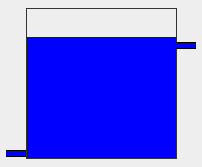
\includegraphics[width=90pt]{tank.png}
	\end{frame}

	\begin{frame}
		\frametitle{Exercises}
		\begin{enumerate}
			\item Complete the simulation program (from \url{https://github.com/wbombardellis/java-unterricht/tree/master/Programme/09/simulation})
		\end{enumerate}
	\end{frame}

	\begin{frame}
		\frametitle{For Grammar Rules}
		$for\ (\langle \text{Statement 1} \rangle; \langle \text{Boolean Condition} \rangle; \langle \text{Statement 3} \rangle)\ \{$\\
			\cindent $...$\\
		$\}$\\
		\begin{itemize}
			\item \emph{Statement 1} is executed (one time) before the execution of the code block.
			\item \emph{Boolean Condition} defines the condition for executing the code block.
			\item \emph{Statement 3} is executed (every time) after the code block has been executed.
		\end{itemize}
	\end{frame}

	\begin{frame}
		\frametitle{Exercises}
		\begin{enumerate}
			\item Write a program that calculates the geometric series \[\sum_{n=1}^{N}{z^n}\] for any z. Verify that, for $z=\frac{1}{2}$, it converges to $1$ as $N \to \infty$.
			\pause
			\item Extend the previous program to also calculate the alternating harmonic series $ \sum_{n=1}^{N}{\frac{(-1)^{n-1}}{n}}$ and verify that it converges to $ln(2)$ as $N \to \infty$.
		\end{enumerate}
	\end{frame}

	\begin{frame}
		\frametitle{Exercises}
		\begin{enumerate}
			\item Write a program that calculates the factorial of a number. The factorial of a positive integer n, denoted by $n!$, is $n \cdot (n-1) \cdot (n-2) \cdots 1$. Additionally, $0! = 1$.
			\pause
			\item Write a program that prints the following pattern up to a desired N.\\
			\texttt{1\\
				1 2\\
				1 2 3\\
				1 2 3 4\\
				$\vdots$\\
				1 2 3 4 5 $\cdots$ N}
		\end{enumerate}
	\end{frame}

	%-------------------
	% Summary
	%-------------------
	\section{Summary}
	
	\begin{frame}
		\frametitle{Summary}
		\begin{itemize}
			\item For allows you to execute the same code several times
			\item Next Lesson: Arrays
		\end{itemize}
	\end{frame}

	\begin{frame}
		\frametitle{References}
		\begin{itemize}
			\item W3C Tutorial: 
			\begin{itemize}
				\item \url{https://www.w3schools.com/java/java_for_loop.asp}
			\end{itemize}
			\item Exercises: \url{https://www.w3schools.com/java/exercise.asp}
			\begin{itemize}
				\item Java Loops
			\end{itemize}
		\end{itemize}
		
	\end{frame}

\end{document}
